\documentclass[border=2mm]{standalone}
\usepackage{tikz}
\usepackage{mathtools}
% \usepackage{tikz-3dplot}
\usetikzlibrary{calc}

\begin{document}
% \tdplotsetmaincoords{70}{120}

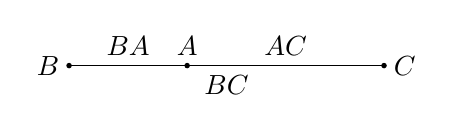
\begin{tikzpicture}[>=stealth]
  \coordinate (B) at (0,0);
  \coordinate (A) at (1.5,0);
  \coordinate (C) at (4,0);

  \draw[-] (B) -- (A) node[midway, above] {$BA$};

  \draw[-] (A) -- (C) node[midway, above] {$AC$};

  \draw[-] (B) -- (C) node[midway, below] {$BC$};

  \fill (B) circle (1pt) node[left] {$B$};

  \fill (A) circle (1pt) node[above] {$A$};

  \fill (C) circle (1pt) node[right] {$C$};
\end{tikzpicture}

\end{document}